\begin{abcliste}
\abc With $a$ the side of the triangle: the charges have opposite signs, so the up quark attracts the down quark with
\begin{align}
 F_1 &= \FaF \\
   &= \kC\times\frac{\frac{2}{9}\times\left(\qe\right)^2}{\left(\sq\right)^2} \\
   &= \Fa \approx \result{\FaP{0}{2}}
\end{align}

\abc
\begin{center}
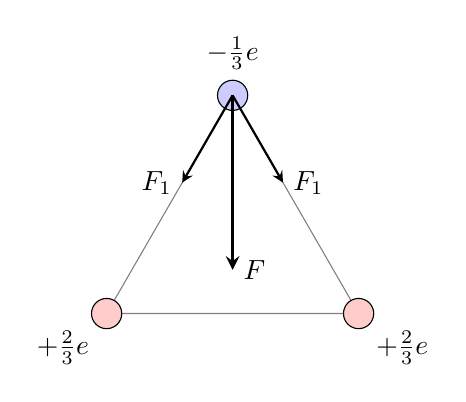
\begin{tikzpicture}[>=stealth, scale=1.6]
 \draw[gray] (-1,0) -- (1,0) -- (0,1.732) -- cycle;
 \draw[fill=red!20] (-1,0) circle (0.12) node[below left=1mm] {$+\frac{2}{3}e$};
 \draw[fill=red!20] (1,0) circle (0.12) node[below right=1mm] {$+\frac{2}{3}e$};
 \draw[fill=blue!20] (0,1.732) circle (0.12) node[above=2mm] {$-\frac{1}{3}e$};
 \draw[->, thick] (0,1.732) -- (-0.4,1.039) node[left] {$F_1$};
 \draw[->, thick] (0,1.732) -- (0.4,1.039) node[right] {$F_1$};
 \draw[->, very thick] (0,1.732) -- (0,0.346) node[right] {$F$};
\end{tikzpicture}
\end{center}
The two forces have the same size and are \ang{60} apart, each \ang{30} from the line to the midpoint between the up quarks. Their components across that line cancel, those along it add up:
\begin{align}
 F &= \FF = \sqrt{3}\,F_1 \\
   &= \sqrt{3}\times\Fa \\
   &= \F \approx \result{\FP{0}{2}}
\end{align}
It points from the down quark towards the midpoint between the two up quarks.
\end{abcliste}
